\subsection{Content Server} \label{section:counter-replace-server}
An approach to fight the shortcomings of the license verification libraries is moving it to a server.
The introduction service managed accounts, users have to login on a server in order to verify their license.
Instead of returning the result of the verification, the server delivers the content of the application.
Since the license verification is no longer inside the application \gls{dex} file, Lucky Patcher is not able to manipulate it anymore.
\newline
\begin{figure}[h]
    \centering
    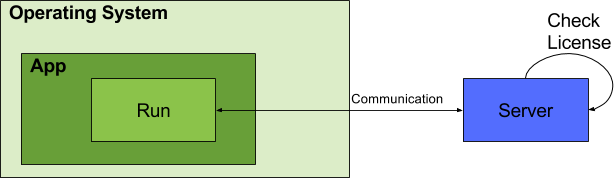
\includegraphics[width=0.8\textwidth]{data/contentServer.png}
    \caption{Abstraction of an application and a content server}
    \label{fig:contentServer}
\end{figure}
The implementation can be described with the application Spotify \cite{spotify} as a reference.
Instead of using local license verification, the user has to enter his credentials, which are send to the server.
In case the credentials are valid, the user is logged into the application.
The content, the music in this case, is no longer on the phone itself, but streamed from the server.
The attacker still can circumvent the user verification inside the application, but they are facing a second layer of security afterwards.
Since the content is on the server and the user has to be authorized on it, no content is available inside the application.
Thus attacks on the applications itself do not work anymore that easily.
\newline
Having a content server is good solution against piracy but it has downsides as well.
The first problem is that this model cannot be applied to all applications universally.
It means that it must be possible to extract parts of the application's logic and implement them on a server.
This is not possible for all applications.
The second problem are the additional resources needed.
When outsourcing parts of the application on a server, not only knowledge and money is needed for the server, but an additional application for the server has to be created as well.
Not every developer can handle this additional workload.
The third problem is the resulting always online necessaty which limits the freedom of users and creates additional unnecessary traffic.
This is not accepted by all users.
\newline
Nevertheless, if this implementation can be realized, it is safe from \gls{luckypatcherg} auto patching as well as custom patches.
In addition, this mechanism protects the developers \gls{ip} when the core algorithm is moved to the server.
This prevents attackers not from only using the application for free, but also from reconstructing the the core functionality and implementing it somewhere else, thus the application gives less incentives for attackers.
